	\section{Preventivo}
	Di seguito verranno inseriti i preventivi e la suddivisione dei ruoli per le varie fasi dello sviluppo. La suddivisione dei ruoli è stata realizzata seguendo i seguenti principi:
	\begin{enumerate}
		\item Ogni membro del gruppo, per spartirsi equamente il carico di lavoro, deve ricoprire tutti i ruoli almeno una volta per un periodo di tempo sufficiente a comprenderne il funzionamento
		\item Il totale delle ore complessivo di ogni membro deve essere compreso tra le 85 e le 105 ore rendicontate
		\item In ogni fase ogni membro del gruppo dovrebbe rendicontare all'incirca lo stesso numero di ore lavorative degli altri membri
	\end{enumerate} 
	Per la realizzazione del preventivo sono stati usati i valori di costo orario indicati alla pagina \url{https://www.math.unipd.it/~tullio/IS-1/2018/Progetto/RO.html} ovvero
	\begin{itemize}
		\item Responsabile \textit{(RES)}: 30\euro/ora
		\item Amministratore \textit{(AMM)}: 20\euro/ora
		\item Analista \textit{(ANA)}: 25\euro/ora
		\item Progettista \textit{(PRO)}: 22\euro/ora
		\item Programmatore \textit{(PRR)}: 15\euro/ora
		\item Verificatore \textit{(VER)}: 15\euro/ora
	\end{itemize}	
	
	\subsection{Attività preliminari di analisi}
	\subsubsection{prospetto orario}
	
		\begin{tabular}{c c c c c c c|c }
			\hline
			\multicolumn{8}{|c|}{\textbf{Suddivisione ruoli in ore}}\\
			\hline
			\textbf{Nominativo} & RES & AMM & ANA & PRO & PRR & VER & \textbf{Totale} \\
			\hline
			Matteo Bordin\\
			\hline
			Pietro Casotto\\
			\hline
			Michele Clerici\\
			\hline
			Marco Davanzo\\
			\hline
			Davide Liu\\
			\hline
			Davide Ghiotto\\
			\hline
			Gianluca Pegoraro\\
			\hline

		\end{tabular}
	
	\subsubsection{conteggio ore}
		\begin{tabular}{ c c c}
			\hline
			\multicolumn{3}{|c|}{\textbf{Suddivisione ruoli in ore}}\\
			\hline
			\textbf{Ruolo} & Ore & Costo\\
			\hline
			\textbf{Responsabile} \\
			\hline
			\textbf{Amministratore} \\
			\hline
			\textbf{Analista} \\
			\hline
			\textbf{Progettista} \\
			\hline
			\textbf{Programmatore}  \\
			\hline
			\textbf{Verificatore} \\
			\hline 
		\end{tabular}

	
	\subsection{Consolidamento dei requisiti}
	\subsubsection{prospetto orario}
	\subsubsection{conteggio ore}

	
	\subsection{Progettazione di dettaglio e codifica}
	\subsubsection{Prospetto orario}
	La distribuzione oraria della fase di Progettazione di dettaglio e codifica è la seguente:
	
\begin{table}[!htpb]
	\centering
	\renewcommand{\arraystretch}{2} 
	\rowcolors{2}{gray!25}{white}
	\begin{tabular}{|l c c c c c c|c| }
		\rowcolor{orange!50}
		\hline
		\multicolumn{8}{|c|}{\textbf{Suddivisione delle ore nei vari ruoli}}\\
		\hline
		\textbf{Nominativo} & RES 	& AMM 	& ANA 	& PRO 	& PRG 	& VER 	& \textbf{Totale} \\
		\hline
		\mat  				& 8		& -		& -		& -		& 22	& 6		& 36\\
		\hline
		\pie  				& -		& -		& -		& 16	& 20	& -		& 36\\
		\hline
		\mic  				& -		& -		& -		& 16	& 20	& -		& 36\\
		\hline
		\mar  				& 8		& -		& -		& -		& 12	& 16		& 36\\
		\hline
		\daG  				& -		& 12	& -		& -		& 14 	& 10		& 36\\
		\hline
		\daL  				& -		& -		& -		& 10	&20		& 6		& 36\\
		\hline
		\gia  				& -		& 12	& -		&12		& -		& 12	& 36\\
		\hline
	\end{tabular}
	\caption{Suddivisione ore del periodo di Progettazione di dettaglio e codifica}
\end{table}
	Di seguito rappresentata anche in un grafico:
\begin{figure}[!htpb]
	\centering
	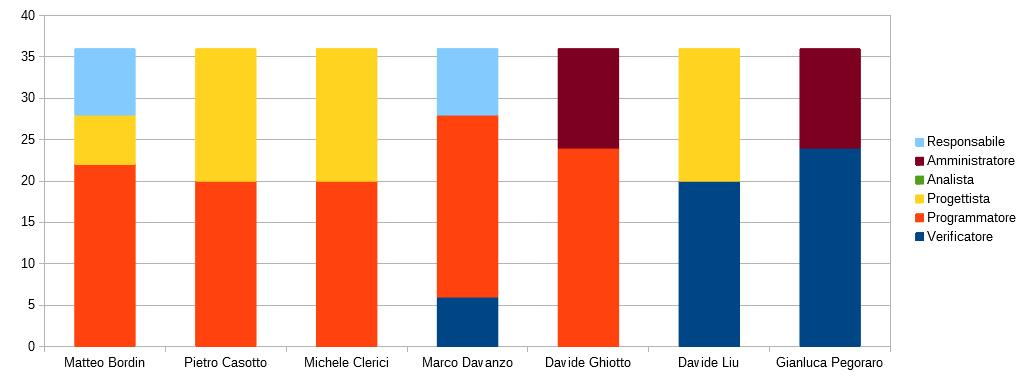
\includegraphics[width=\textwidth]{preventivo/grafico_terza_parte.jpg}
	\caption{Grafico suddivisione oraria nel periodo di Progettazione di dettaglio e codifica}
\end{figure}

\subsubsection{Conteggio ore}
	La distribuzione delle ore nei vari ruoli nella fase di Progettazione di dettaglio e codifica è la seguente:
	
\begin{table}[!htpb]
	\centering
	\renewcommand{\arraystretch}{2} 
	\rowcolors{2}{gray!25}{white}
	\begin{tabular}{| c c c|}
		\rowcolor{orange!50}
		\hline
		\multicolumn{3}{|c|}{\textbf{Suddivisione ruoli in ore}}\\
		\hline
		\textbf{Ruolo} 			& Ore 	& Costo\\
		\hline
		\textbf{Responsabile}	&16		&480\\
		\hline
		\textbf{Amministratore}	&24		&480\\
		\hline
		\textbf{Analista}		&0		&0\\
		\hline
		\textbf{Progettista}	&54		&1188\\
		\hline
		\textbf{Programmatore}	&108	&1620\\
		\hline
		\textbf{Verificatore} 	&50		&750\\
		\hline
		\textbf{Totale} 		&252	&4518\\
		\hline 
	\end{tabular}
	\caption{Ore e costi totali del periodo di Progettazione di dettaglio e codifica}
\end{table}
	Di seguito rappresentata anche in un grafico:
\begin{figure}[!htpb]
	\centering
	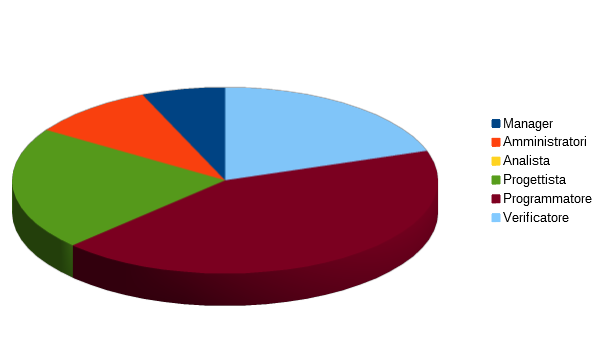
\includegraphics[scale=0.7]{preventivo/torta_terza_parte.png}
	\caption{Grafico suddivisione ruoli nel periodo di Progettazione di dettaglio e codifica}
\end{figure}
\clearpage
	
	\subsection{Validazione e collaudo}
	\subsubsection{Prospetto orario}
	La distribuzione oraria della fase di Validazione e collaudo è la seguente:
	
	\begin{table}[!htpb]
		\centering
		\renewcommand{\arraystretch}{2} 
		\rowcolors{2}{gray!25}{white}
		\begin{tabular}{|l c c c c c c|c| }
			\rowcolor{orange!50}
			\hline
			\multicolumn{8}{|c|}{\textbf{Suddivisione delle ore nei vari ruoli}}\\
			\hline
			\textbf{Nominativo} & RES 	& AMM 	& ANA 	& PRO 	& PRG 	& VER 	& \textbf{Totale} \\
			\hline
			\mat  				&-		& 12	&-		&-		&-		& 9		&21 \\
			\hline
			\pie  				&-		& 12	&-		&-		&-		& 9		&21\\
			\hline
			\mic  				&-		&-		&-		&-		& 6		& 15	&21\\
			\hline
			\mar  				&-		&-		&-		&-		& 10	& 11	&21\\
			\hline
			\daG  				& 8		&-		&-		&-		&-		& 13	&21\\
			\hline
			\daL  				&-		&-		&-		&-		&-		& 21	&21\\
			\hline
			\gia  				& 8		&-		&-		&-		&-		& 13	&21\\
			\hline
		\end{tabular}
		\caption{Suddivisione ore del periodo di Validazione e collaudo}
	\end{table}
	~\newline
	Di seguito rappresentata anche in un grafico:
\begin{figure}[!htpb]
	\centering
	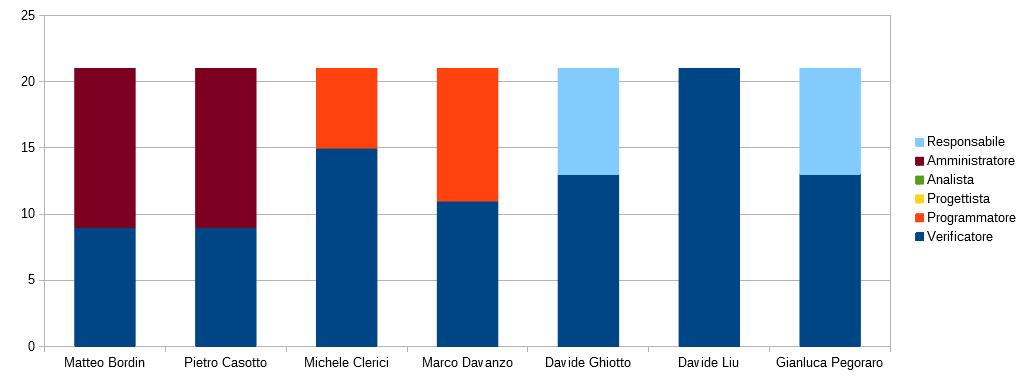
\includegraphics[width=\textwidth]{preventivo/grafico_quarta_parte.jpg}
	\caption{Grafico suddivisione oraria nel periodo di Validazione e collaudo}
\end{figure}
	\newpage
	\subsubsection{Conteggio ore}
	La distribuzione delle ore nei vari ruoli nella fase di Validazione e collaudo è la seguente:
	
	\begin{table}[!htpb]
			\centering
		\renewcommand{\arraystretch}{1.8} 
		\rowcolors{2}{gray!25}{white}
		\begin{tabular}{| c c c|}
			\rowcolor{orange!50}
			\hline
			\multicolumn{3}{|c|}{\textbf{Suddivisione delle ore nei vari ruoli}}\\
			\hline
			\textbf{Ruolo} 			& Ore 	& Costo\\
			\hline
			\textbf{Responsabile}	&16		&480\\
			\hline
			\textbf{Amministratore}	&24		&480\\
			\hline
			\textbf{Analista}		&0		&0\\
			\hline
			\textbf{Progettista}	&0		&0\\
			\hline
			\textbf{Programmatore}	&16		&240\\
			\hline
			\textbf{Verificatore} 	&91		&1365\\
			\hline
			\textbf{Totale} 		&147	&2565\\
			\hline 
		\end{tabular}
		\caption{Ore e costi totali del periodo di Validazione e collaudo}
	\end{table}
	~\newline Di seguito rappresentata anche in un grafico:
\begin{figure}[!htpb]
	\centering
	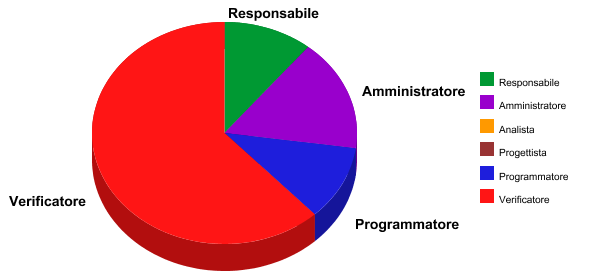
\includegraphics[scale=0.8]{preventivo/torta_quarta_parte.png}
	\caption{Grafico suddivisione ruoli nel periodo di Validazione e collaudos}
\end{figure}
\clearpage

